% version 1.2 dated 09 May 2011

% This file (c) 2009-2011 Elsevier Ltd.  Modifications may be freely made,
% provided the edited file is saved under a different name

% This file contains modifications for Procedia Computer Science

% Changes since version 1.1
% - added "procedia" option compliant with ecrc.sty version 1.2a
%   (makes the layout approximately the same as the Word CRC template)
% - added example for generating copyright line in abstract

%-----------------------------------------------------------------------------------

%% This template uses the elsarticle.cls document class and the extension package ecrc.sty
%% For full documentation on usage of elsarticle.cls, consult the documentation "elsdoc.pdf"
%% Further resources available at http://www.elsevier.com/latex

%-----------------------------------------------------------------------------------

%%%%%%%%%%%%%%%%%%%%%%%%%%%%%%%%%%%%%%%%%%%%%%%%%%%%%%%%%%%%%%
%%%%%%%%%%%%%%%%%%%%%%%%%%%%%%%%%%%%%%%%%%%%%%%%%%%%%%%%%%%%%%
%%                                                          %%
%% Important note on usage                                  %%
%% -----------------------                                  %%
%% This file should normally be compiled with PDFLaTeX      %%
%% Using standard LaTeX should work but may produce clashes %%
%%                                                          %%
%%%%%%%%%%%%%%%%%%%%%%%%%%%%%%%%%%%%%%%%%%%%%%%%%%%%%%%%%%%%%%
%%%%%%%%%%%%%%%%%%%%%%%%%%%%%%%%%%%%%%%%%%%%%%%%%%%%%%%%%%%%%%

%% The '3p' and 'times' class options of elsarticle are used for Elsevier CRC
%% The 'procedia' option causes ecrc to approximate to the Word template
\documentclass[3p,times,procedia]{elsarticle}
\flushbottom

%% The `ecrc' package must be called to make the CRC functionality available
\usepackage{ecrc}
\usepackage{parskip}
\usepackage{amsmath}
\usepackage{ragged2e}
\usepackage{graphicx}
\usepackage{float}
\usepackage{listings}
\usepackage{color}

\usepackage{soul}

% \lstset{basicstyle=\ttfamily, keywordstyle=\bfseries}
\definecolor{mygreen}{rgb}{0,0.6,0}
\definecolor{mygray}{rgb}{0.5,0.5,0.5}
\definecolor{mymauve}{rgb}{0.58,0,0.82}

\lstset{ %
  backgroundcolor=\color{white},   % choose the background color
  basicstyle=\scriptsize,        % size of fonts used for the code
  breaklines=true,                 % automatic line breaking only at whitespace
  captionpos=b,                    % sets the caption-position to bottom
  commentstyle=\color{mygreen},    % comment style
  escapeinside={\%*}{*)},          % if you want to add LaTeX within your code
  keywordstyle=\color{blue},       % keyword style
  stringstyle=\color{mymauve},     % string literal style
}



\definecolor{darkred}{rgb}{0.6,0.0,0.0}
\definecolor{darkgreen}{rgb}{0,0.50,0}
\definecolor{lightblue}{rgb}{0.0,0.42,0.91}
\definecolor{orange}{rgb}{0.99,0.48,0.13}
\definecolor{grass}{rgb}{0.18,0.80,0.18}
\definecolor{pink}{rgb}{0.97,0.15,0.45}

% listings
\usepackage{listings}

% General Setting of listings
\lstset{
  aboveskip=1em,
  breaklines=true,
  abovecaptionskip=-6pt,
  captionpos=b,
  escapeinside={\%*}{*)},
  frame=single,
%   numbers=left,
  numbersep=15pt,
  numberstyle=\tiny,
}
% 0. Basic Color Theme
% \lstdefinestyle{colored}{ %
%   basicstyle=\ttfamily,
%   backgroundcolor=\color{white},
%   commentstyle=\color{green}\itshape,
%   keywordstyle=\color{blue}\bfseries\itshape,
%   stringstyle=\color{red},
% }
% 1. General Python Keywords List
\lstdefinelanguage{PythonPlus}[]{Python}{
  morekeywords=[1]{,as,assert,nonlocal,with,yield,self,True,False,None,} % Python builtin
  morekeywords=[2]{,__init__,__add__,__mul__,__div__,__sub__,__call__,__getitem__,__setitem__,__eq__,__ne__,__nonzero__,__rmul__,__radd__,__repr__,__str__,__get__,__truediv__,__pow__,__name__,__future__,__all__,}, % magic methods
  morekeywords=[3]{,object,type,isinstance,copy,deepcopy,zip,enumerate,reversed,list,set,len,dict,tuple,range,xrange,append,execfile,real,imag,reduce,str,repr,}, % common functions
  morekeywords=[4]{,Exception,NameError,IndexError,SyntaxError,TypeError,ValueError,OverflowError,ZeroDivisionError,}, % errors
  morekeywords=[5]{,ode,fsolve,sqrt,exp,sin,cos,arctan,arctan2,arccos,pi, array,norm,solve,dot,arange,isscalar,max,sum,flatten,shape,reshape,find,any,all,abs,plot,linspace,legend,quad,polyval,polyfit,hstack,concatenate,vstack,column_stack,empty,zeros,ones,rand,vander,grid,pcolor,eig,eigs,eigvals,svd,qr,tan,det,logspace,roll,min,mean,cumsum,cumprod,diff,vectorize,lstsq,cla,eye,xlabel,ylabel,squeeze,}, % numpy / math
}
% 2. New Language based on Python
\lstdefinelanguage{PyBrIM}[]{PythonPlus}{
  emph={d,E,a,Fc28,Fy,Fu,D,des,supplier,Material,Rectangle,PyElmt},
}
% 3. Extended theme
\lstdefinestyle{colorEX}{
  basicstyle=\ttfamily,
  backgroundcolor=\color{white},
  commentstyle=\color{darkgreen}\slshape,
  keywordstyle=\color{blue}\bfseries\itshape,
  keywordstyle=[2]\color{blue}\bfseries,
  keywordstyle=[3]\color{grass},
  keywordstyle=[4]\color{red},
  keywordstyle=[5]\color{orange},
  stringstyle=\color{darkred},
  emphstyle=\color{pink}\underbar,
}



\newcommand{\subf}[2]{%
  {\small\begin{tabular}[t]{@{}c@{}}
  #1\\#2
  \end{tabular}}%
}

%% The ecrc package defines commands needed for running heads and logos.
%% For running heads, you can set the journal name, the volume, the starting page and the authors

%% set the volume if you know. Otherwise `00'
%%\volume{}

%% set the starting page if not 1
\firstpage{1}

%% Give the name of the journal
\journalname{Computational Intelligence, Spring 2022}

%% Give the author list to appear in the running head
%% Example \runauth{C.V. Radhakrishnan et al.}
\runauth{}

%% The choice of journal logo is determined by the \jid and \jnltitlelogo commands.
%% A user-supplied logo with the name <\jid>logo.pdf will be inserted if present.
%% e.g. if \jid{yspmi} the system will look for a file yspmilogo.pdf
%% Otherwise the content of \jnltitlelogo will be set between horizontal lines as a default logo

%% Give the abbreviation of the Journal.
%% \jid{}

%% Give a short journal name for the dummy logo (if needed)
%\jnltitlelogo{Computer Science}

%% Hereafter the template follows `elsarticle'.
%% For more details see the existing template files elsarticle-template-harv.tex and elsarticle-template-num.tex.

%% Elsevier CRC generally uses a numbered reference style
%% For this, the conventions of elsarticle-template-num.tex should be followed (included below)
%% If using BibTeX, use the style file elsarticle-num.bst

%% End of ecrc-specific commands
%%%%%%%%%%%%%%%%%%%%%%%%%%%%%%%%%%%%%%%%%%%%%%%%%%%%%%%%%%%%%%%%%%%%%%%%%%

%% The amssymb package provides various useful mathematical symbols

\usepackage{amssymb}
%% The amsthm package provides extended theorem environments
%% \usepackage{amsthm}

%% The lineno packages adds line numbers. Start line numbering with
%% \begin{linenumbers}, end it with \end{linenumbers}. Or switch it on
%% for the whole article with \linenumbers after \end{frontmatter}.
%% \usepackage{lineno}

%% natbib.sty is loaded by default. However, natbib options can be
%% provided with \biboptions{...} command. Following options are
%% valid:

%%   round  -  round parentheses are used (default)
%%   square -  square brackets are used   [option]
%%   curly  -  curly braces are used      {option}
%%   angle  -  angle brackets are used    <option>
%%   semicolon  -  multiple citations separated by semi-colon
%%   colon  - same as semicolon, an earlier confusion
%%   comma  -  separated by comma
%%   numbers-  selects numerical citations
%%   super  -  numerical citations as superscripts
%%   sort   -  sorts multiple citations according to order in ref. list
%%   sort&compress   -  like sort, but also compresses numerical citations
%%   compress - compresses without sorting
%%
%% \biboptions{authoryear}

% \biboptions{}

% if you have landscape tables
\usepackage[figuresright]{rotating}
%\usepackage{harvard}
% put your own definitions here:x
%   \newcommand{\cZ}{\cal{Z}}
%   \newtheorem{def}{Definition}[section]
%   ...

% add words to TeX's hyphenation exception list
%\hyphenation{author another created financial paper re-commend-ed Post-Script}

% declarations for front matter


\begin{document}
\begin{frontmatter}

%% Title, authors and addresses

%% use the tnoteref command within \title for footnotes;
%% use the tnotetext command for the associated footnote;
%% use the fnref command within \author or \address for footnotes;
%% use the fntext command for the associated footnote;
%% use the corref command within \author for corresponding author footnotes;
%% use the cortext command for the associated footnote;
%% use the ead command for the email address,
%% and the form \ead[url] for the home page:
%%
%% \title{Title\tnoteref{label1}}
%% \tnotetext[label1]{}
%% \author{Name\corref{cor1}\fnref{label2}}
%% \ead{email address}
%% \ead[url]{home page}
%% \fntext[label2]{}
%% \cortext[cor1]{}
%% \address{Address\fnref{label3}}
%% \fntext[label3]{}

%\dochead{Middle East Technical University, Spring 2023}%

%% Use \dochead if there is an article header, e.g. \dochead{Short communication}
%% \dochead can also be used to include a conference title, if directed by the editors
%% e.g. \dochead{17th International Conference on Dynamical Processes in Excited States of Solids}

\title{\textbf{Saving the Princess with a \\ Reinforcement Learning Agent}}

%% use optional labels to link authors explicitly to addresses:
%% \author[label1,label2]{<author name>}
%% \address[label1]{<address>}
%% \address[label2]{<address>}



\author[]{Ozgur Gulsuna} 
%\author[b]{Second Author}
%\author[a,b]{Third Author\corref{cor1}}

\address[]{Middle East Technical University, Electrical and Electronics Engineering, Ankara, Turkey}
%\address[b]{Second affiliation, Address, City and Postcode, Country}

\begin{abstract}
%% Text of abstract
This report explores the reinforcement learning processes and applies it to a challenging task that is playing Mario. Two main algorithms are experimented with
Proximal Policy Optimization (PPO) and Deep Q-Networks (DQN) are compared in terms of their hyperparametes and performance.
The temporal interfacing layer is implemented with Cnn and Mlp and comparison based on prior knowledge is made.
The figures are visualized with Tensorboard and the results are discussed.
\end{abstract}

\begin{keyword}
PyTorch;
 NumPy;
 Reinforcement Learning;
 SuperMarioBros;
 PPO;
 DQN;
 Tensorboard;
\end{keyword}

\end{frontmatter}

%\correspondingauthor[*]{Corresponding author. Tel.: +0-000-000-0000 ; fax: +0-000-000-0000.}
\email{ozgur.gulsuna@metu.edu.tr}

%%
%% Start line numbering here if you want
%%
% \linenumbers

%% main text

\enlargethispage{10mm}
\section{\textbf{Basic Questions}}
\label{main}



% \subsection{\textbf{Agent}}

\begin{enumerate}
    \item \textbf{Agent:} The agent is the entity that interacts with the environment. It tries to maximize the reward it can acquire. In our case, the agent is the Mario character. In supervisied learning the agent can be the model that is trained with the data. \\
    \item \textbf{Environment:} The environment is the world in which the agent lives. In other words, the system is the environment, it consist of problems or rewards. In our case, the environment is the Super Mario Bros game. In supervised learning the closest thing to the environment can be the data that is used to train the model. \\
    \item \textbf{Reward:} The reward is the feedback that the agent receives from the environment. In each state the reward is calculated and the agent learns upon that reward trying to increase it. In our case, the reward is the score that Mario gets from the game. In supervised learning the reward can be the loss function that is used to train the model. \\
    \item \textbf{Policy:} The policy is the series of mappings acting as a "strategy" that the agent uses to determine the next action. In our case, the policy is the strategy that Mario uses to determine the next action. In supervised learning policy does not exist. \\
    \item \textbf{Exploration:} The exploration is the process of the agent trying to find the best policy. In our case, the exploration is the process of Mario trying to find the best strategy to get the highest score. In supervised learning the exploration can be the process of the model trying to find the best parameters to minimize the loss function. \\
    \item \textbf{Exploitation:} The exploitation is the process of the agent using the best policy it found and not altering it but perfecting. In our case, the exploitation is the process of Mario tweaking the best strategy it has found to get the highest score but it does not search for a complete new strategy. In supervised learning a comparible term does not exist. \\
\end{enumerate}

\vspace{-0.5em}

% \subsection{\textbf{Gradient Computation}}
% High number of iterations, when the difference between the weights are small, the gradient calculation can be made with basic slope calculation.
% \vspace{-0.7em}
% \begin{equation*}
%     \begin{array}{l}
%          \textrm{$ \textstyle  \gamma \nabla \mathcal{L}_{\omega_{k}} = \omega_{k} - \omega_{k+1}  $} \\
%         \hspace{10em} hence, \\
%          \displaystyle \textrm{$  \nabla_{\omega} \mathcal{L}\big\rvert_{\omega = \omega_{k}} = \frac{\omega_{k} - \omega_{k+1}}{\gamma}$}   \\
%     \end{array}
% \end{equation*}

% \subsection{\textbf{Some Training Parameters and Basic Parameter Calculations}}
% \begin{enumerate}
%     \item The batch refers to a subset of the training data that is used to compute the weights for one iteration. More specifically, the batch size is the number of training samples in a batch.
%  The epoch on the other hand refers to the number of times the entire training data is used to update the weights. In training, there are generally multiple epoch iterations where the weights are updated with different batches/subsets of the training data.
%     \item For the $N$ number of training samples, the number of batches per epoch is $N/B$, where $B$ is the batch size. A little side note that the solution is rounded up to the higher integer if $N/B$ is not an integer.
%     \item For the optimization iterations, such as SGD, for $E$ number of epochs, the total number of iterations is $E \times N/B$. Again, a practical side note states that the $N/B$ is rounded up to the higher integer.
% \end{enumerate}
% \subsection{\textbf{Computing Number of Parameters of ANN Classifiers}}
% \begin{enumerate}
%     \item Starting from the initial layer of the MLP, we have $D_{in}$ number of input neurons and $H_1$ number of neurons in first hidden layer. Also there are biases associated with 
% each neuron. Therefore, the number of parameters of the each layer is,
%     \vspace{-0.5cm}
%     \begin{equation*}
%     \begin{array}{r}
%     \textrm{Input Layer} = D_{in} \times H_{1} \ +\ H_{1} \\
%     \textrm{Hidden Layers}= H_1 \times H_2 + H_2\\
%     \cdot \cdot \cdot \hspace{2em} \\
%     \textrm{More Hidden Layers} = H_{k-1} \times H_k + H_k\\
%     \textrm{Output Layer} = H_{k} \times D_{out} \ +\ D_{out} \\
%     \end{array}
%     \end{equation*}

%     \vspace{-0.25cm}
%     The total sum can be written as, where $K$ is the number of hidden layers.
%     \vspace{-0.5cm}
%     \begin{equation*}
%         \textrm{Total Number of Parameters} = D_{in}\times H_1 + \sum_{k=2}^{K} (H_{k-1} \times H_k + H_k) + H_k \times D_{out} +  D_{out}
%     \end{equation*}
%     \vspace{-0.25cm}

%     \item CNN structure is more complicated. The number of parameters of a CNN layer is calculated as follows:
    
%     For the input layer, the number of parameters is,
%     \vspace{-0.5cm}
%     \begin{equation*}
%         \textrm{Input Layer} = [(H_{in}-H_1+1) \times (W_{in}-W_1+1)\times C_{in} \times C_1 ]+ C_1
%     \end{equation*}

%     \vspace{-0.25cm}
%     where $H_{in}$ and $W_{in}$ are the height and width of the input image, and $C_{in}$ is the number of channels of the input image.
%     Each input of layer is the output of the previous layer.
%     There exist also biases associated with each neuron added.
%     For the convolutional layers, the number of parameters is calculated as,
%     \vspace{-0.5cm}
%     \begin{equation*}
%         \begin{array}{c}
%             \displaystyle \textrm{Convolutional Layer} = [(H_k-H_{k+1}+1) \times (W_k-W_{k+1}+1) \times C_{k} \times C_{k+1}] + C_{k+1} \\
%             \\
%             \displaystyle \textrm{Combination of all layers is,} \\
%             \displaystyle \textrm{Convolutional Layers} = \sum_{k=1}^{K} [(H_k-H_{k+1}+1) \times (W_k-W_{k+1}+1) \times C_{k} \times C_{k+1}] + C_{k+1} \\ 
%         \end{array}
%     \end{equation*}

%     \vspace{-0.25cm}
%     Here all the parameters are summed up. The output is assumed to be the last index of the array.
%     The final equation for the total number of parameters is,
%     \vspace{-0.5cm}

    
%     \begin{equation*}
%         \hspace{-1cm} \textrm{Total Parameters} = [(H_k-H_{k+1}+1) \times (W_k-W_{k+1}+1) \times C_{k} \times C_{k+1}] + C_{k+1} + \sum_{k=1}^{K} [(H_k-H_{k+1}+1) \times (W_k-W_{k+1}+1) \times C_{k} \times C_{k+1}] + C_{k+1}
%     \end{equation*}

%     \vspace{-0.25cm}

% \end{enumerate}

% All tables should be numbered with Arabic numerals. Every table should have a caption. Headings should be placed above tables, left justified. Only horizontal lines should be used within a table, to distinguish the column headings from the body of the table, and immediately above and below the table. Tables must be embedded into the text and not supplied separately. Below is an example which the authors may find useful.

% \begin{table}[h]
% \caption{ An example of a table.}
% \begin{tabular*}{\hsize}{@{\extracolsep{\fill}}lll@{}}
% \toprule
% An example of a column heading & Column A ({\it{t}}) & Column B ({\it{t}})\\
% \colrule
% And an entry &   1 &  2\\
% And another entry  & 3 &  4\\
% And another entry &  5 &  6\\
% \botrule
% \end{tabular*}
% \end{table}

% %\enlargethispage{12pt}

\section{\textbf{Benchmarking}}

\subsection{\textbf{PPO}}
The subjects of the experiments considering the PPO algorithm are the following.
Each column represents hyperparamters of that algorithm. The hyperparameters are as follows:

% \begin{itemize}
%     \item \textbf{Tag:} \hspace{5em} PPO\textunderscore1, PPO\textunderscore2, PPO\textunderscore3
%     \item \textbf{Policy:} 'CnnPolicy', 'CnnPolicy', 'CnnPolicy'
%     \item \textbf{Learning Rate:} 0.000001, 0.0001, 0.000001
%     \item \textbf{Preprocessing:} 4 Stack, 4 Stack, 8 Stack
%     \item \textbf{Preprocessing:} Grayscale, Grayscale, Grayscale
% \end{itemize}

\begin {table}[H]
\begin{center}
\begin{tabular}{c|c|c|c|c}
\hline
\textbf{Tag} & \textbf{Policy} & \textbf{Learning Rate} & \textbf{Preprocessing} & \textbf{Preprocessing} \\
\hline
\hline
PPO\textunderscore1 & 'CnnPolicy' & 0.000001 & 4 Stack & Grayscale \\
\hline
PPO\textunderscore2 & 'CnnPolicy' & 0.0001 & 4 Stack & Grayscale \\
\hline
PPO\textunderscore3 & 'CnnPolicy' & 0.000001 & 8 Stack & Grayscale \\
\hline
\end{tabular}
\end{center}
\end {table}


\vspace{-2em}
\begin{figure}[H]
    \centering
    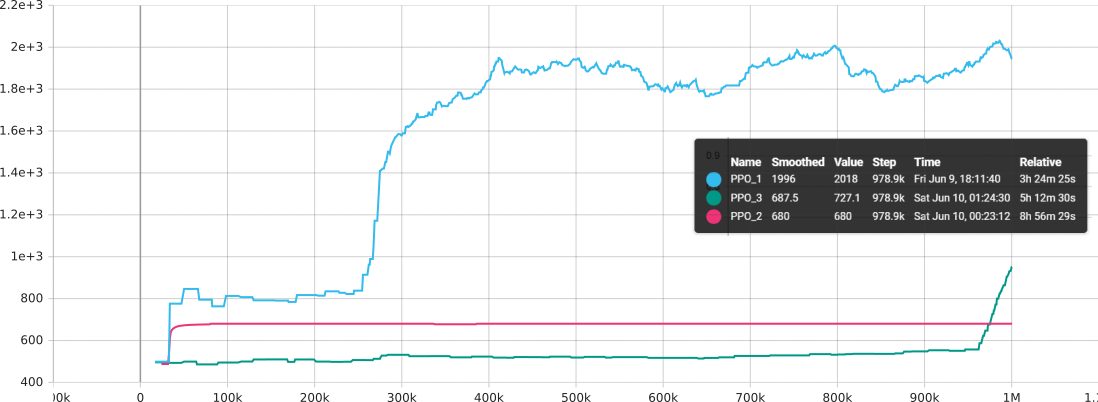
\includegraphics[width=0.85\textwidth]{figures/PPO-REW.png}
    \caption{r\_ep\_rew\_mean vs timesteps (1M)}
\end{figure}


\vspace{-2.5em}
\begin{figure}[H]
    \centering
    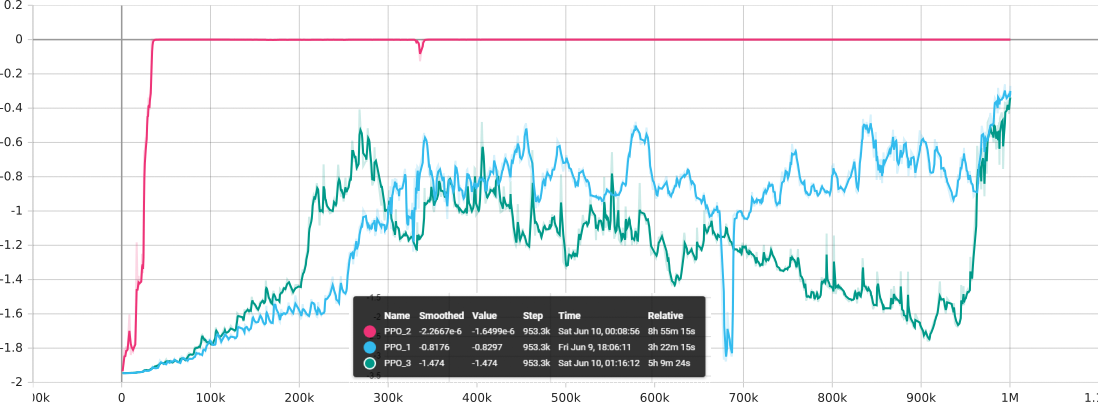
\includegraphics[width=0.85\textwidth]{figures/PPO-ENT.png}
    \caption{entropy\_loss vs timesteps (1M)}
\end{figure}


\subsection{\textbf{DQN}}
The subjects of the experiments considering the DQN algorithm are the following.
Each column represents hyperparamters of that algorithm. The hyperparameters are as follows:

% \begin{itemize}
%     \item \textbf{Tag:} \hspace{5em} PPO\textunderscore1, PPO\textunderscore2, PPO\textunderscore3
%     \item \textbf{Policy:} 'CnnPolicy', 'CnnPolicy', 'CnnPolicy'
%     \item \textbf{Learning Rate:} 0.000001, 0.0001, 0.000001
%     \item \textbf{Preprocessing:} 4 Stack, 4 Stack, 8 Stack
%     \item \textbf{Preprocessing:} Grayscale, Grayscale, Grayscale
% \end{itemize}

\begin {table}[H]
\begin{center}
\begin{tabular}{c|c|c|c|c}
\hline
\textbf{Tag} & \textbf{Policy} & \textbf{Batch Size} & \textbf{Preprocessing} & \textbf{Buffer Size} \\
\hline
\hline
DQN\textunderscore2 & 'CnnPolicy' & 192 & 4 Stack & 10000 \\
\hline
DQN\textunderscore4 & 'CnnPolicy' & 192 & 4 Stack & 20000 \\
\hline
DQN\textunderscore1 & 'CnnPolicy' & 192 & 8 Stack & 10000 \\
\hline
\end{tabular}
\end{center}
\end {table}


\vspace{-2em}
\begin{figure}[H]
    \centering
    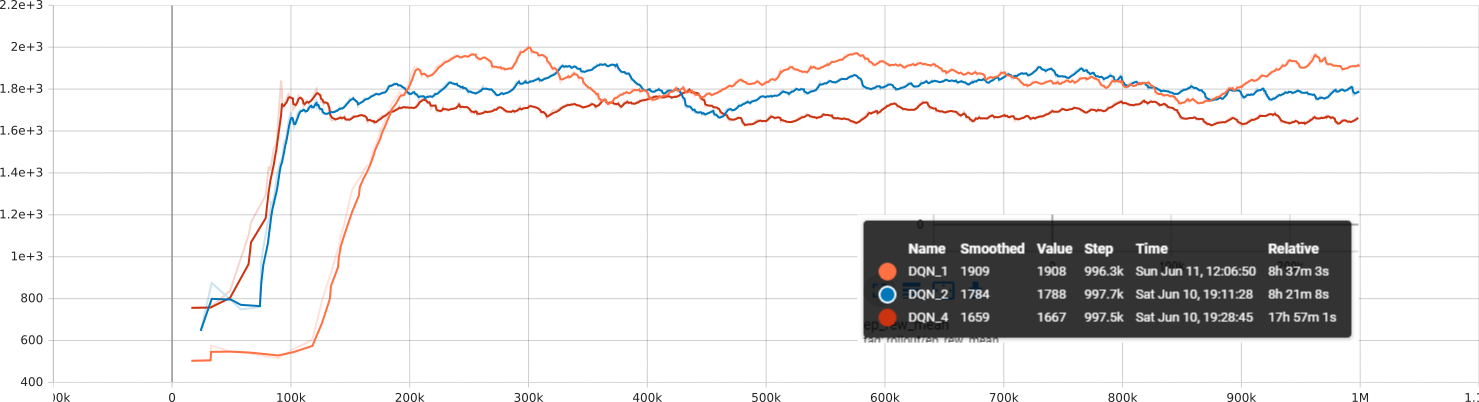
\includegraphics[width=0.85\textwidth]{figures/DQN_REW.png}
    \caption{r\_ep\_rew\_mean vs timesteps (1M)}
\end{figure}


\vspace{-2.5em}
\begin{figure}[H]
    \centering
    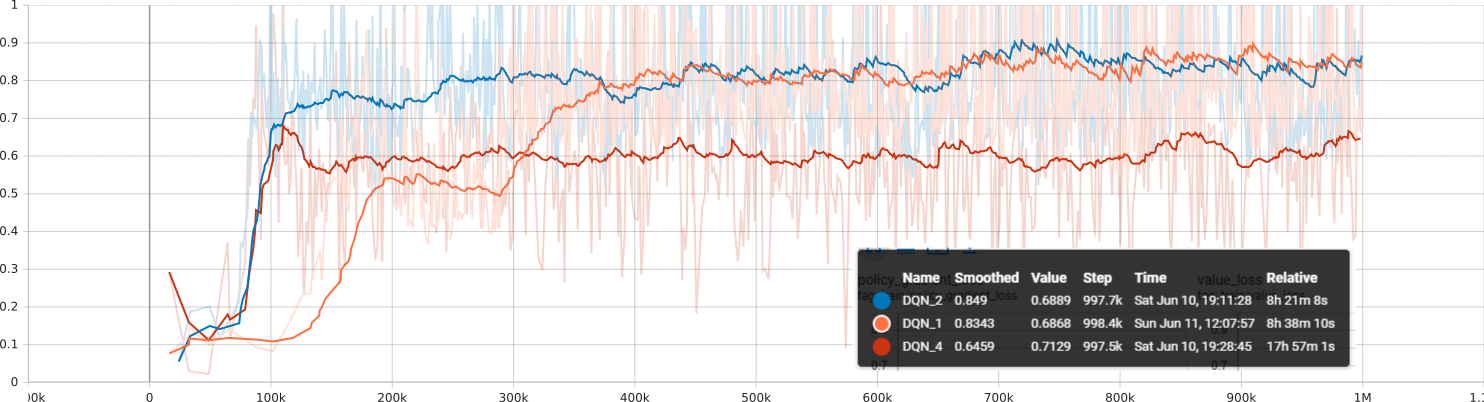
\includegraphics[width=0.85\textwidth]{figures/DQN_LOSS.png}
    \caption{loss vs timesteps (1M)}
\end{figure}



\subsection{\textbf{Comparison}}
The comparison of the two algorithms is shown in the following figures.


\begin{figure}[H]
    \centering
    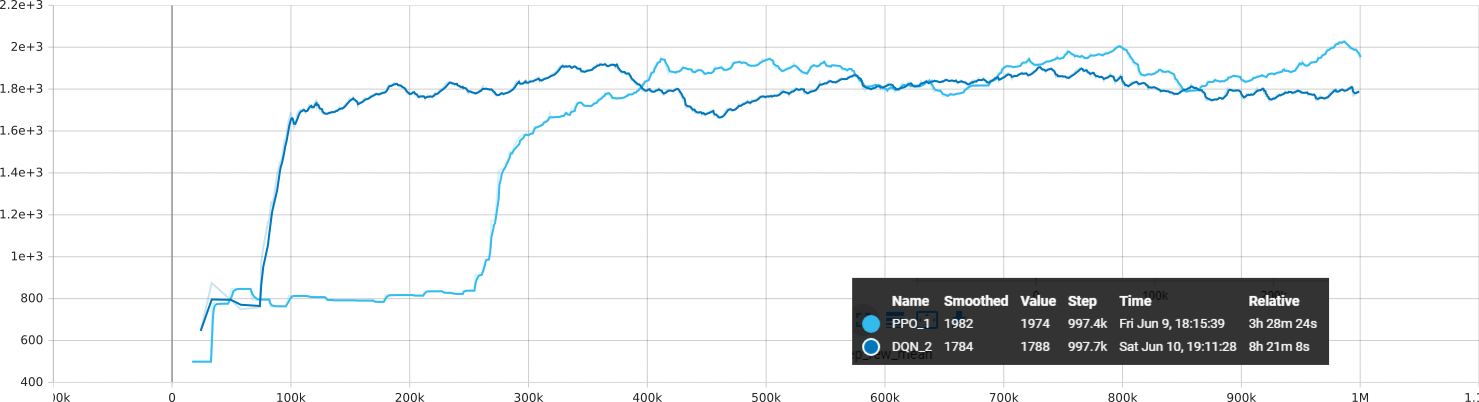
\includegraphics[width=0.85\textwidth]{figures/COMP_REW.png}
    \caption{r\_ep\_rew\_mean vs timesteps (1M)}
\end{figure}


\vspace{-2.5em}
\begin{figure}[H]
    \centering
    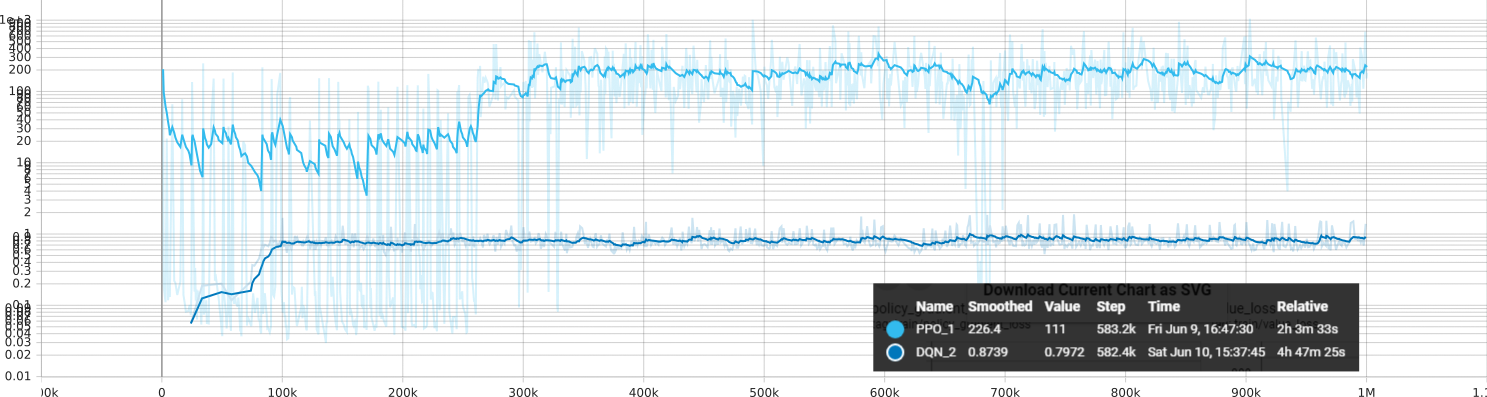
\includegraphics[width=0.85\textwidth]{figures/COMP_LOSS.png}
    \caption{loss vs timesteps (1M)}
\end{figure}


\section{\textbf{Discussions}}
\vspace{3em}
\begin{enumerate}
    \item Mario struggles to jump over the pipes up to the iteration number between 100000 and 200000. At around 200000 it can get points from blocks and killing enemies at maximum it could get 700 points. In this time period it did not explored much to get points from blocks nor it knows the question marked blocks. 
    \\
    \item DQN is shown to be perform better faster than PPO. But on the end they both saturated around the same reward. When we compare the training time, PPO is trained faster than DQN. Then it is a matter of computation power on the training time.
    \\
    \item Exploration and exploitation performance can be compared with the reward plot. The DQN exploit more hence it converges faster but the peak performance is limited. PPO explores more and it converge more slow but the peak performance is higher than DQN.
    \\
    \item In terms of generalization performance, both algoritms are seem to be performing bad. The DQN is little bit better than PPO. PPO likes to jump continuously in places that it is not familiar with. Again it is not easily observer but DQN is little bit better than PPO in terms of both generalization and adaptation.
    \\
    \item Only a couple hyperparameters are compared.
    Starting with the PPO, default parameters worked best, increased learning rate made the performance worse. 
    In terms of preprocessing stack size increased to 8 made the training take longer hence its performance can not be compared since it needed more training steps.
    \\

    On the DQN case, in terms of reward buffersize does not make a difference.
    when the losses are compared in buffersize experiment, the 20000 buffer size is better than 10000 buffer size. The higher the buffersize more the RAM required for the training process.
    In terms of stack size, 8 stack size has a better end game performance but again it took more timesteps to train.
    \\
    \item DQN consist of deep Q-networks and the training process is more computationally expensive than PPO. The training performance shows that although it is slower to train, it learned in less steps to play Mario. The practical comparison tell us that PPO is better for more "realtime" applications where DQN is better for more "offline" applications.
    \\
    \item Comparison of 'MlpPolicy' and 'CnnPolicy' without making an experimentation is possible since it is known that for more complex temporal inputs such as complex game screen, the 'CnnPolicy' is better since it can understand the important aspects of the complex imputs such as enemies and different textured blocks. The 'MlpPolicy' is more suited to clean binary type inputs.
\end{enumerate}


\section{\textbf{Performance}}
Watch @ https://youtu.be/vjRhMvMw6Xc

% \begin{figure}[H]
%     \centering
%     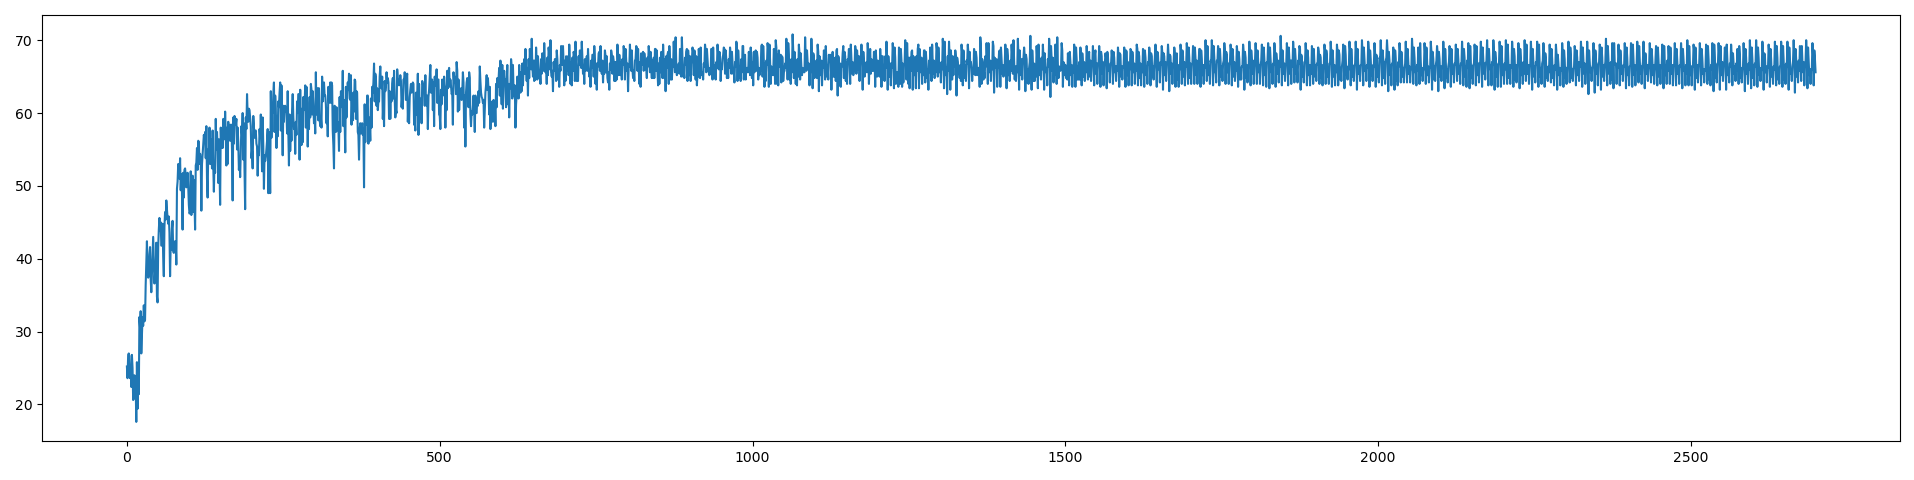
\includegraphics[width=0.95\textwidth, trim={0 1cm 0 1cm}]{figures/cnn_4_SC_validation_acc.png}
%     \caption{Validation Accuracy with Scheduled Learning Rate for the "cnn\_4".} 
%     \label{fig:SC}
% \end{figure}

% \begin{figure}[H]
%     \centering
%     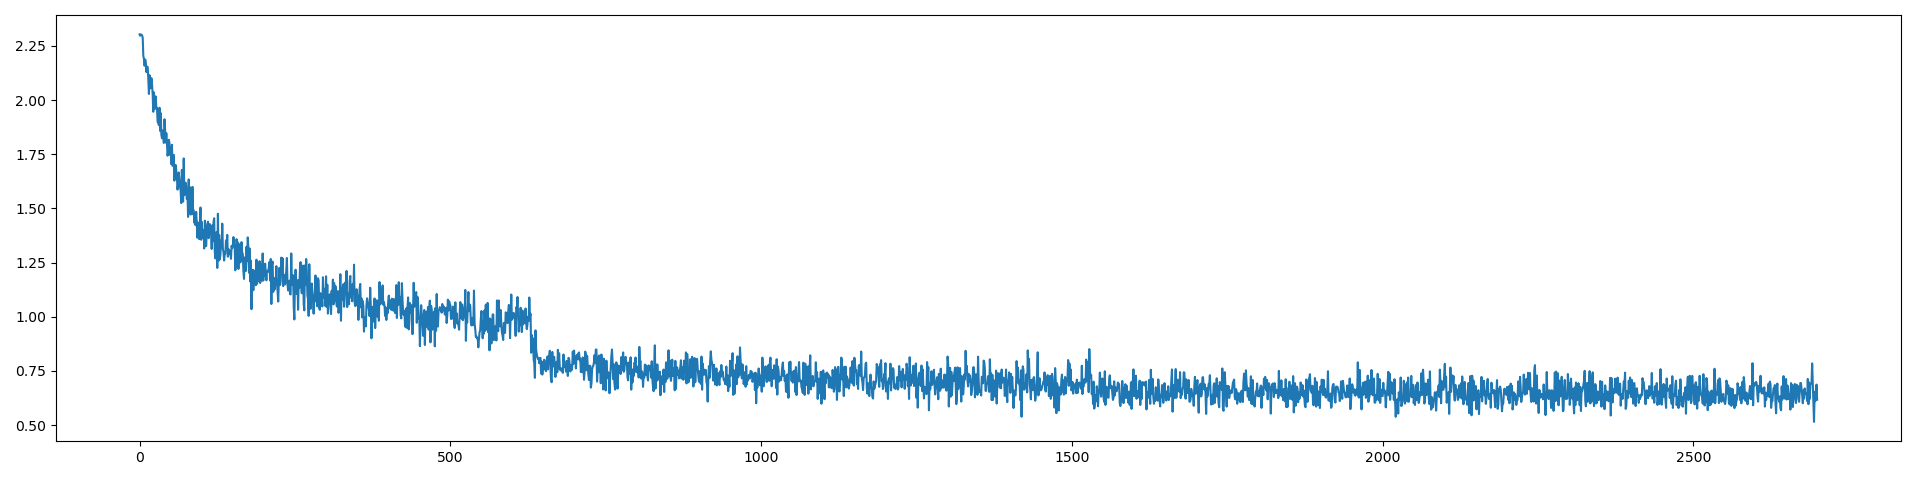
\includegraphics[width=0.95\textwidth, trim={0 1cm 0 1cm}]{figures/cnn_4_SC_training_loss.png}
%     \caption{Training Loss with Scheduled Learning Rate for the "cnn\_4".} 
%     \label{fig:SC2}
% \end{figure}

% Please title your files in this order `procedia acronym\_conference acronym\_authorslastname'.  Submit both the source file and the PDF to the Guest Editor.

% Artwork filenames should comply with the syntax ``aabbbbbb.ccc'', where:
% \begin{itemize}
% \item a = artwork component type
% \item b = manuscript reference code
% \item c = standard file extension

% Component types:
% \item gr = figure
% \item pl = plate
% \item sc = scheme
% \item fx = fixed graphic
% \end{itemize}


% \subsection{Footnotes}
% Footnotes should be avoided if possible. Necessary footnotes should be denoted in the text by consecutive superscript letters\footnote{Footnote text.}. The footnotes should be typed single spaced, and in smaller type size (8 pt), at the foot of the page in which they are mentioned, and separated from the main text by a one line space extending at the foot of the column. The `Els-footnote' style is available in the ``TeX Template'' for the text of the footnote.

% Please do not change the margins of the template as this can result in the footnote falling outside printing range.


% \section{Illustrations}
% All figures should be numbered with Arabic numerals (1,2,3,$\,\ldots.$). Every figure should have a caption. All\break photographs, schemas, graphs and diagrams are to be referred to as figures. Line drawings should be good\break quality scans or true electronic output. Low-quality scans are not acceptable. Figures must be embedded into the text and not supplied separately. In MS word input the figures must be properly coded. Preferred format of figures are PNG, JPEG, GIF etc. Lettering and symbols should be clearly defined either in the caption or in a legend provided as part of the figure. Figures should be placed at the top or bottom of a page wherever possible, as close as possible to the first reference to them in the paper. Please ensure that all the figures are of 300 DPI resolutions as this will facilitate good output.

% The figure number and caption should be typed below the illustration in 8 pt and left justified [{\bfseries\itshape Note:} one-line captions of length less than column width (or full typesetting width or oblong) centered]. For more guidelines and\break information to help you submit high quality artwork please visit: http://www.elsevier.com/artworkinstructions\break Artwork has no text along the side of it in the main body of the text. However, if two images fit next to each other, these may be placed next to each other to save space. For example, see Fig.~1.
% \begin{figure}[t]\vspace*{4pt}
% %\centerline{\includegraphics{fx1}\hspace*{5mm}\includegraphics{fx1}}
% %\centerline{\includegraphics{gr1}}
% \caption{(a) first picture; (b) second picture.}
% \end{figure}


% \section{Equations}
% Equations and formulae should be typed in MathType, and numbered consecutively with Arabic numerals in parentheses on the right hand side of the page (if referred to explicitly in the text). They should also be separated from the surrounding text by one space
% \begin{equation}
% \begin{array}{lcl}
% \displaystyle X_r &=& \displaystyle\dot{Q}^{''}_{rad}\left/\left(\dot{Q}^{''}_{rad} + \dot{Q}^{''}_{conv}\right)\right.\\[6pt]
% \displaystyle \rho &=& \displaystyle\frac{\vec{E}}{J_c(T={\rm const.})\cdot\left(P\cdot\left(\displaystyle\frac{\vec{E}}{E_c}\right)^m+(1-P)\right)}
% \end{array}
% \end{equation}


% \section{Online license transfer}
% All authors are required to complete the Procedia exclusive license transfer agreement before the article can be published, which they can do online. This transfer agreement enables Elsevier to protect the copyrighted material for the authors, but does not relinquish the authors' proprietary rights. The copyright transfer covers the exclusive rights to reproduce and distribute the article, including reprints, photographic reproductions, microfilm or any other reproductions of similar nature and translations. Authors are responsible for obtaining from the copyright holder, the permission to reproduce any figures for which copyright exists.

% \section*{Acknowledgements}

% Acknowledgements and Reference heading should be left justified, bold, with the first letter capitalized but have no numbers. Text below continues as normal.

% %% The Appendices part is started with the command \appendix;
% %% appendix sections are then done as normal sections
% %% \appendix

% %% \section{}
% %% \label{}

% \appendix
% \section{Python Scripts}


% \subsection{Example of a sub-heading within an appendix}
% There is also the option to include a subheading within the Appendix if you wish.
%% References
%%
%% Following citation commands can be used in the body text:
%% Usage of \cite is as follows:
%%   \cite{key}         ==>>  [#]
%%   \cite[chap. 2]{key} ==>> [#, chap. 2]
%%

%The citation must be used in following style: \cite{article-minimal} \cite{article-full} \cite{article-crossref} \cite{whole-journal}.
%% References with BibTeX database:

%\bibliography{xampl}
%\bibliographystyle{elsarticle-harv}


%% Authors are advised to use a BibTeX database file for their reference list.
%% The provided style file elsarticle-num.bst formats references in the required Procedia style

%% For references without a BibTeX database:

%  \begin{thebibliography}{}

%% \bibitem must have the following form:
%%   \bibitem{key}...
%%

% \bibitem{Massimo2011}
% {F}ilippini, Massimo, and Lester C. Hunt. (2011) ``Energy demand and
% energy efficiency in the OECD countries: a stochastic demand frontier
% approach." {\it Energy Journal} {\bf 32} (2): 59--80.
% \bibitem{Massimo2012}
% Filippini, Massimo, and Lester C. Hunt. (2012) ``US residential
% energy demand and energy efficiency: A stochastic demand frontier
% approach." {\it Energy Economics} {\bf 34} (5): 1484--1491.
% \bibitem{Thomas2015} 
% Weyman-Jones, Thomas, J\'{u}lia Mendon\c{c}a Boucinha, and Catarina
% Feteira In\'{a}cio. (2015) ``Measuring electric energy efficiency in
% Portuguese households: a tool for energy policy." {\it Management of Environmental Quality: An International Journal} {\bf 26} (3): 407--422.
% \bibitem{} 
% Saunders, Harry (2009) ``Theoretical Foundations of the Rebound Effect'', in Joanne Evans and Lester Hunt (eds) {\it International Handbook on the Economics of Energy}, Cheltenham, Edward Elgar
% \bibitem{} 
% Sorrell, Steve (2009) ``The Rebound Effect: definition and estimation'', in Joanne Evans and Lester Hunt (eds) {\it International Handbook on the Economics of Energy}, Cheltenham, Edward Elgar 
%  \end{thebibliography}

\clearpage

%%%% This page is for instructions only, once the article is finalize please omit the below text before creating the final PDF
\normalMode

% \section*{Instructions to Authors for LaTeX template:}

% \section{ZIP mode for LaTeX template:}

% The zip package is created as per the guide lines present on the URL http://www.elsevier.com/author-schemas/ preparing-crc-journal-articles-with-latex for creating the LaTeX zip file of Procedia LaTeX template.  The zip generally contains the following files:
% \begin{Itemize}[]\leftskip-17.7pt\labelsep3.3pt
% \item ecrc.sty
% \item  elsarticle.cls
% \item elsdoc.pdf
% \item .bst file
% \item Manuscript templates for use with these bibliographic styles
% \item  Generic and journal specific logos, etc.
% \end{Itemize}

% The LaTeX package is the main LaTeX template. All LaTeX support files are required for LaTeX pdf generation from the LaTeX template package. 

% {\bf Reference style .bst file used for collaboration support:} In the LaTeX template packages of all Procedia titles a new ``.bst'' file is used which supports collaborations downloaded from the path http://www.elsevier.com/author-schemas/the-elsarticle-latex-document-class

% \section{Reference style used in Computer Science:}
% \let\footnotesize\normalsize
% \hspace*{-10pt}\begin{tabular*}{\hsize}{@{}ll@{}}
% {\bf Title}&{\bf Reference style} \\[6pt]
% PROCS  & 3 Vancouver Numbered
% \end{tabular*}

\end{document}

%%
%% End of file `procs-template.tex'.
